\chapter{State of the Art} \label{ch:State of the Art}
In this chapter we explain the fundamental theory of Functional Reactive Programming and approaches in debugging applications that use this pattern. We also examine existing debugging tools that target Reactive Programming frameworks and libraries as well as Reactive Programming libraries for JavaScript. We discuss the Chrome Reactive Inspector (CRI) and work targeting CRI prior to this thesis in detail in addition to its main competitor RxFiddle.

\section{Implementation of Reactive Systems}
	\subsection{Reactive Functional Programming}
	A Reactive Functional Programming \cite{FRP} (from now on \emph{Reactive Programming}) framework or library removes a lot of boilerplate code the developer usually has to implement to propagate changes and event throughout a software system. It advances the well known Observer Design Pattern and overcomes several short-comings of that approach. In the Observer Design Pattern, a Subject propagates changes to its state to a list of prior registered Observers. In contrast to an Observable (also called Behavior) in Reactive Programming, which can provide multiple values over time as a stream, a Subject can only return one value - its state.
	In addition to Observables which provide varying values over time, a Reactive Programming implementation usually contains a possibility to handle discrete events over time called Events or Event Streams\cite{BaconJS}.
	
	What we refer to as an Observable actually consists of three parts - a Producer that produces values over time, the actual Observable that stores these values, and the Observer that notifies all Subscribers (sometimes also called Consumers). The notification of the Subscribers is specific to \emph{push-based} systems where the values are pushed through the reactive system when a new value arrives, rather than being pulled in a pull-based system on demand if a value is requested by a Subscriber of an Observable or any of its descendants (other Observables that depend upon it).
	Observables can also be categorized as \emph{hot} or \emph{cold} \cite{HotVsCold}. A \emph{cold} Observable will create a new Producer each time a Subscriber subscribes to its Observer. The Producer will be destroyed when the Subscriber unsubscribes - this is referred to as the unicast approach. On the other hand all Subscribers to a \emph{hot} Observable will (usually) share one Producer - this is referred to as the multicast approach.
	
	The declarative functional programming style limits side-effects and is usually implemented with many \emph{pure} functions as operators that can be used to transform, combine or change behavior of Observables and Event Streams. The operators return a new Observable that depends upon the Observable on which the operator was used. Using these operators, the developer declares dependencies between observables, which creates more comprehensible program code and structure \cite[Why Reactive Programming?]{ReactiveInspector} than imperative programming style would produce. 	


	\subsection{RxJS and BaconJS}
	Although there are many JavaScript implementations of the reactive design pattern like Cycle\cite{CycleJS}, Kefir\cite{KefirJS} or  Most\cite{MostJS}, this section is focused on ReactiveX for JavaScript (RxJS) \cite{RxJS} and Bacon (BaconJS) \cite{BaconJS}, because these are the libraries the Chrome Reactive Inspector currently supports. A comprehensible list of reactive frameworks and libraries for JavaScript can be found at \cite{FRPJSList}.
	
	\textbf{Rx.js}\\
	Reactive Extensions for JavaScript or RxJS is the JavaScript implementation of ReactiveX. There are also ReactiveX implementations for many programming languages, for example Java (RxJava), Scala(RxScala) or C\#(Rx.NET). In extension to the basic concepts of Reactive Programming, RxJS implements Subjects and Schedulers. A Subject represents the implementation of an Event Stream and is the only possibility to realize a multicast Observable, since Observables are \emph{cold} Observables in RxJS They can be Observer and Observable at the same time. To convert a \emph{cold} Observable into a \emph{hot} one the functions \emph{share} or \emph{publish} can be used which will internally use a Subject to track the shared Producer. A Subject will terminate once the last Subscriber unsubscribes. Schedulers are centralized dispatchers that are used to control concurrency that allow to influence the scheduling behavior when asynchronous functions are called e.g. \emph{setTimeout}\cite{RxJsDocu}.
	Observers raise special events if the Observable is completed or reaches an error state - the Observable will not be reusable after wards (even if it is a Subject), which is a main difference to the later discussed BaconJS. RxJS provides many utility functions to convert values, arrays or events into observables \cite{ThesisBaradur}. A basic example of RxJS code to show the general structure can be seen in listing \ref{lst:Rx} (Source: \cite{RxJsDocu} under manual/overview.HTML).
	The latest stable version of RxJS is version 5.5.6 with version 6.0.0-alpha already under active development. RxJS is licensed under the Apache 2.0 license and the source code is publicly available on GitHub \cite{RxJS}.

	\begin{lstlisting}[language=JavaScript, caption={Example of RxJS code.},label={lst:Rx}]
	var button = document.querySelector('button');
	Rx.Observable.fromEvent(button, 'click')
	.throttleTime(1000)
	.scan(count => count + 1, 0)
	.subscribe(count => console.log(`Clicked ${count} times`));
	\end{lstlisting}
	
	\textbf{Bacon.js}\\
	The basic concepts of BaconJS \cite{BaconJS} are Properties - which represent the Observables - and EventStreams that handle distinct events. 
	In contrast to RxJS, BaconJS's Properties are always \emph{hot} Observables. In addition an Error in a EventStream or Property will not cause it to terminate. Errors are therefore handled as any other value which provides more fine grained control for the developer. However, the \emph{endOnError} function can be used if the termination is desired. 
	Another advantage of BaconJS is the \emph{spy} function, which can be used to observe the internal workings and greatly reduces the required effort to create complementary tooling like CRI or RxFiddle. It can also be used to easily create extensive logging without modifying the rest of the reactive application source code. According to the author(s), BaconJS was started because they got frustrated with RxJS, because its source code was not publicly available at the time and the documentations was minimal. They also claim that BaconJS has a more consistent and glitch free stream/property behavior \cite{BaconJSRepo}, but they also explain that RxJS has less overhead and therefore a better performance. 
		\begin{lstlisting}[language=JavaScript, caption={Example of BaconJS code.},label={lst:Bacon}]
	$("#username input").asEventStream("keyup")
	.map(function(event) {
	return $(event.target).val();
	})
	.toProperty("")
	\end{lstlisting}
	The latest stable version of BaconJS is version 2.0.0 and it is still under active development. BaconJS is licensed under the MIT license and the source code is publicly available on GitHub \cite{BaconJSRepo}.

	While BaconJS is a newer Reactive Programming library and was developed to handle some short-comings of RxJS, according to the GitHub statistics RxJS has still a much larger community. RxJS has 387 watches, 10540 stars, 991 forks and 185 contributors for the currently active repository and BaconJS has 156 watches, 5839 stars, 328 forks and 83 contributors in total (last accessed: 31.1.2018 18:22).
	In addition, since RxJS started earlier and due to its similarity to other ReactiveX implementations in other languages, there exist a multitude of tools and utility libraries that are exclusive for RxJS - including RxFiddle.

\subsection{Debugging Reactive Code}
The violation of a syntax rule of in a programming language such as missing control characters, misspelled keywords etc. are syntax errors and can be detected by most IDEs very precisely, but logical errors are harder to track down. Modern IDEs use breakpoints including conditional breakpoints, step by step execution, event logging, stack traces and many more. Due to reactive programming being declarative, breakpoints, the most useful feature for in-depth code and state inspection at a precise point during the applications execution can not be used as easily. For some IDE even chained function calls (also called Method chaining \cite{MethodChaining}) provide an obstacle, because there breakpoints are line- and not character position based. But even if the IDE can handle breakpoints inside anonymous functions for the usual navigation features like \emph{Step Over} and \emph{Step Into} it is not trivial to balance between providing the necessary fine grained stepping and having to many steps for the developer to iterate. For example one of the most advanced IDEs there is, Visual Studio (2017) for .NET, will step over the whole batch of chained functions if the developer uses \emph{Step Over}, but will step into the first anonymous function in the chain if the developer uses \emph{Step Into}. The developer can then use \emph{Step Over} to enumerate the anonymous functions passed to the chained functions (see listing \ref{lst:CSharp_LINQ}). This is a very specialized and desirable behavior that will match the intend of the developer most times when using the .Net Framework built in \emph{.NET Language-Integrated Query Expressions} (LINQ), but this behavior will break as soon as a custom function is added to the chain (\emph{DoCustom} in the code example). Now the \emph{Step Into} on line 1 will step into \emph{DoCustom} for each entry in the list and will then step out of the batch of chained functions to line 10. If a similar code example in BaconJS is debugged with the step-by-step debugging feature of Google Chrome, it will actually step through the BaconJS library code even if the developer just uses \emph{Step Over}. Because BaconJS or other reactive programming libraries are not part of native JavaScript Google Chrome has no means to determine if the user wants to step through the library code or not.
This example shows that debugging declarative code is still a hard task for modern IDEs, especially if Out-of-Order execution (LINQ Expressions are executed Out-of-Order) is added.
The developers intention is not easy to interpret by the IDE, because there is a multitude of possible steps to take there. The developer could want to debug the custom chained function, they could want to iterate the anonymous functions passed as arguments to the chained functions, they could also want to step through the framework functions (Select, Where, OrderBy, etc. which is possible if framework debugging is enabled in Visual Studio 2017 for .NET). 
For big collections, or in the case of reactive programming, observables with many submitted values this problem is also increased by having too many single executions of a anonymous function for the developer to step through. Another example for this is a breakpoint inside a anonymous function that is passed to a declarative function (like\emph{Where} in C\# or \emph{map} in BaconJS) which halts the application for each element in the collection or data stream.

%TODO: language is c# but the compilation would not complete with "[Sharp]C" as language.
\begin{lstlisting}[language=JavaScript, caption={Simple example of .NET LINQ in C\# to show the steps the Visual Studio 2017 for .NET debugger takes while debugging step-by-step.},label={lst:CSharp_LINQ}]
 var lst = new List<string>{"test1","test2"};
 var result = lst.Select(s => s.ToUpper())
 .Where(s =>
 {
	var b = s.StartsWith("t");
	return !b && s.StartsWith("T");
 })
.OrderBy(s => s)
.DoCustom()
.ToList();
\end{lstlisting}


This shows that a traditional debugger is not suitable to use with declarative programming especially reactive programming. While the Visual Studio debugger is still somewhat useful to debug LINQ in .Net, because multiple specialized behaviors have been implemented over the years and LINQ expressions will most likely not cover the entire application and are often used to execute short tasks inside an imperative program flow, observables in a reactive application are usually much more intertwined and make up the general flow of the program; making a traditional debugger more of an obstacle.

As described in \cite{MSDN_DebugginObservables} reverting to the most basic debugging technique sometimes called \emph{printf-debugging} (or in the RxJS terms \emph{do-debugging}), to generate debug outputs or traces by directly modifying the source code, generally provides better results than using advanced features of a traditional debugger. Some shortcomings of this basic technique can be mitigated by using sophisticated tools like shown in \cite{ShinyGraphFromLog} in the section "The Reactive Log" where the log of an application is visualized in a Dependency Graph containing code pieces as nodes. Do-debugging still requires modification of the original source code to trace the programs execution path and pollutes it with statements that do not contribute to the program logic itself, making the code harder to read. \cite{PaperReactiveProgramming} describe the main issue to be missing abstractions and a "mismatch in the mental model", because traditional debuggers operate mainly on the runtime stack information and "do not consider any other abstraction within the running code" \cite{ThesisAbbas}. Traditional debuggers therefore make it very hard for the developer to detect flaws in dependencies between Reactive entities.

In the programming language JavaScript (JS) it is, unlike in compiled languages, by design harder to detect errors in the written code, because it is an interpreted script language and the JS code is not compiled before execution. The general advantage of a script language being able to change the code at runtime and omitting the computation time needed to compile an application, are shadowed by the fact that many bugs can only be found at runtime as well. In addition Type-safe languages can detect many errors even before compilation by verifying that the used types are compatible. This makes Reactive applications written in JavaScript even harder to debug than their counterparts in other languages.

Currently there are few tools to help the developer debug reactive applications and apart from RxFiddle (described in detail in section \ref{sec:RxFiddle}) non of them, as far as we known, support debugging reactive JavaScript applications. One of those tools is \cite{ShinyGraphFromLog} as mentioned above. Another is the Reactive Inspector for the Scala language \cite{ReactiveInspector} started and maintained by Prof. Dr. Guido Salvaneschi working in the Software Technology Group of the Technical University of Darmstadt, Germany.
The Reactive Inspector is an extension of the Scala WIDE for Eclipse. Many features and the basic concepts that are implemented in the \emph{Chrome Reactive Inspector(CRI)} originate from the Reactive Inspector; including the representation of observables and their dependencies in a Dependency Graph called \emph{Reactive Tree}, the possibility to query the history of said %TODO can "said" be used?
 graph or the possibility to search for a specific node in the current graph. They are described in details in section \ref{sec:PreviousCRI}. One main feature of the Reactive Inspector, called \emph{Tree Outline} where the user can quickly jump to different areas of the Dependency Graph, which is useful for applications with large graphs, is currently not implemented for the CRI.

\section{Previous work on the CRI and its main competitor}
In this section we will cover the previous work on the Chrome Reactive Inspector (CRI) as well as RxFiddle which is the main competitor for the CRI because both have a similar goal to help developers debug Reactive Systems in JavaScript with abstract concepts that go beyond traditional debugging.

	\subsection{The Chrome Reactive Inspector}
	\label{sec:PreviousCRI}
	The Chrome Reactive Inspector is based on the Reactive Inspector for Scala \cite{ReactiveInspector} and was developed by the Software Technology Group at the TU-Darmstadt Germany supervised by Prof. Dr. Guido Salvaneschi. It is implemented as a Google Chrome(Chrome) extension that extends the Chrome Developer Tools (DevTools) with another panel that inspects and instruments a target Reactive Web application that is using RxJS or BaconJS. Prior to this thesis there have already been two Master theses targeting the CRI that provide the base theory and source code of this thesis.\\
	
	\textbf{Master Thesis by Waqas Abbas}\\
	
	\cite{ThesisAbbas} The main goal of the Master Thesis by Waqas Abbas was to develop and implement a concept for a Chrome extension based on the Reactive Inspector to debug Reactive Web applications in JavaScript. One mayor difficulty was to find a viable solution for intercepting calls to the Reactive libraries in order to retrieve the necessary information about observables and their dependencies that are used to build a Dependency Graph (called Dependency Tree in \cite{ReactiveInspector}) as well as to gather additional details like variable name that directly correspond to observables and providing them with context by instrumenting the source code. An in-browser solution taken from a demo page \cite{JalangiDemo} of Jalangi was used to instrument and analyze the source code directly. The main Jalangi framework \cite{Jalangi} is currently not usable solely within a browser.
	Abbas also implemented several features to help the developer navigate and examine the Dependency Graph and its history. In this first version of the CRI, the user could already submit History Queries that search the History of the Graph for specific nodes or events like node creation, update or the creation of a dependency. In addition the user could add Reactive Breakpoints - breakpoints that pause the program execution when a specific event occurs - or search for a node in a large Dependency Graph.
	At the time the CRI supported BaconJS\cite{BaconJS} and parts of RxJS\cite{RxJS}. Abbas also added a first batch of small Web applications that could be used as test applications to manually verify features of CRI.\\		
		
	\textbf{Master Thesis by Pradeep Baradur}\\
	 \cite{ThesisBaradur} The main goal of the Master Thesis by Pradeep Baradur was to add full support for RxJS to CRI, especially all operators and Subjects. Since RxJS does not provide a uniform way to intercept all calls to the library like the BaconJS's \emph{spy} function, this is a hard problem. For the actual implementation details see \cite{ThesisBaradur} or the \emph{rx-interception.js} file in the current version of CRI. Baradur also reworked the loading of the Content Scripts of CRI and instrumentation to only occur once the CRI DevTools panel is opened for an inspected Web application to reduce load on the browser if the tool is not currently used. He also extended the Find Node and History Query features to allow searching for dependents or dependencies of a node. The focus of his thesis in comparison to Abbas's shifted from being mainly a proof of concept to advancing the CRI to be more reliable and ultimately being usable in a production environment. This included rearranging the UI to be more consistent and improving reliability in general as well as adding additional test applications.\\		
		
	\textbf{Merging previous efforts}\\
	Since Waqas Abbas and Pradeep Baradur's works on the CRI partly overlapped and where developed in separate repositories, uniting both works was the first task for the thesis. Due to being developed separately after Baradur's Thesis started, the repositories shared no common history and due to many refactorings and renames in both projects as they advanced, merging the code base was not possible with automated tools and had to be done manually. Tracing the correlation between different changes was not trivial - in part because both theses were focused on advancing the project and less on maintainability and modularization. For this thesis we took the source code of Pradeep Baradur's Thesis as a base and added features that Waqas Abbas developed after Baradur's Thesis had started. The main reason for this is that Baradur removed many bugs and race conditions that happened in some rarer cases of code execution order, in his goal to make CRI more reliable, that were outside of the scope of Abbas's work.
		
	\subsubsection{Exceptional properties of the CRI implementation}
	The special method that is used to intercept the loading of a Web application by dynamically reloading the JavaScripts to allow direct access and replace specified scripts with an instrumented version has several implications that break the usual \emph{isolated world} \cite{GoogleApiContentScripts} of Google Chrome extensions and their Content Scripts. The loading of the inspected HTML is stopped, the HTML file is scanned for references to JavaScript files that are then loaded and on demand instrumented. The scripts are then executed within the context of the Content Script that does the instrumentation. This is necessary so that both the inspected pages own scripts as well as the Content Scripts of CRI that are responsible for the recording of the inner workings of the used Reactive System share the same RxJS or BaconJS instance. But this approach also has some downsides, for example a global variable in one of the inspected pages scripts may also be used in a script of CRI could cause unforeseen errors - e.g. common libraries like jQuery \cite{jQuery} that provide global objects will cause version conflicts. This also implies a potential security risk, because a Chrome extension runs in a \emph{trusted} context and has access to many Chrome APIs (Application programming interfaces) that are not accessible from a normal Web application - the CRI could therefore be manipulated through shared global variables to execute malicious code by an inspected page.
	Another implication of this approach is that CRI has to filter all referenced JS files of the inspected page to exclude all RxJS or BaconJS scripts from the loading process to use its own versions. This will lead to errors if the versions do not match exactly.
	Dynamically loading the scripts that are referenced by the inspected pages HTML also can not handle any module loader without special interception logic. As module loaders are widely used in modern Web applications and are even part of the ECMA6 \cite{ECMA6import} standard as the \emph{import} keyword, this currently imposes a significant limitation on the number of Web applications CRI can be used with. We provide more detail and discuss some of the possible options in chapter \ref{ch:Future}.
	
	
	In addition to the special circumstances due to the dynamically loading of script in the shared context, CRI also uses a Demo \cite{JalangiDemo} in-browser version of the Jalangi \cite{Jalangi} that does not provide the full features of Jalangi. Instead it only contains features used in the Demo - for example the source code position information of functions and variables do not contain the scripts file name. Jalangi itself contains hundreds of analysis customization options that are not included in the in-browser Demo. Another obstacle presented by using the in-browser Demo script is that it is only available in the \emph{minified} version that is hard to read and debug.
	%TODO check all cite if it was compiled correctly
	
	\subsection{RxFiddle}
	\label{sec:RxFiddle} %TODO capitalization
	RxFiddle \cite{RxFiddle} is a tool developed as part of a Master Thesis by Herman Banken at the Delft University of Technology that displays interactive Marble Diagrams for RxJS Web applications. RxFiddle instruments the used RxJS library to collect information about the inner workings of the library. It is available as a Web application at \cite{RxFiddle} and the source code is publicly available at \cite{RxFiddleGitHub} under the MIT license. RxFiddle is the main competitor of CRI as it is the only other tool (that we are aware of) that tackles debugging for Reactive Systems in JavaScript. In RxFiddle the user can run JavaScript code visible on the left (1) and select a node from a simplistic Dependency Graph (2) to view a Marble Diagram showing details of its events, value streams (3), interaction of operators and anonymous functions (4) passed to these operators.
	
	\begin{figure}[!h]
		\centering
		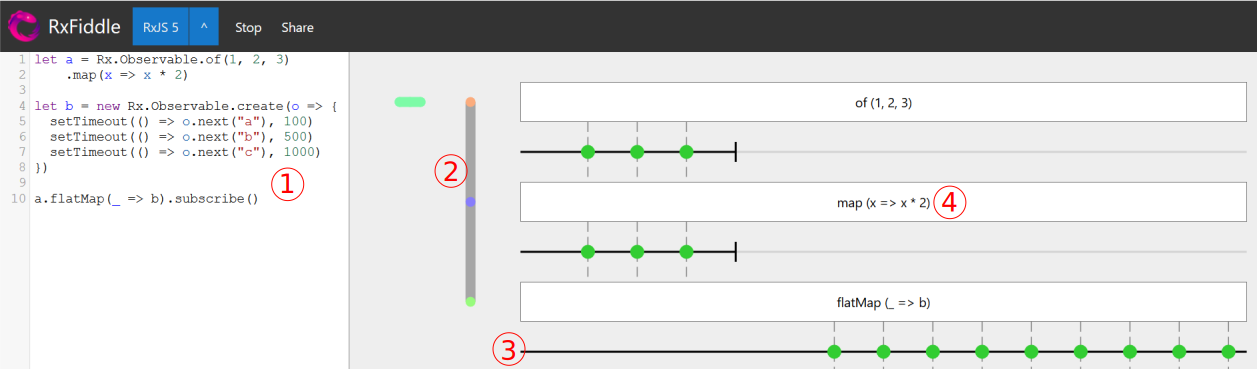
\includegraphics[scale=0.5,trim=0 0 0 0]{gfx/RxFiddleDemo.png}
		\caption{RxFiddle Demo \protect\cite{RxFiddle}}
		\label{fig:RxFiddleDemo}
	\end{figure}

	In the future, the author plans to support multiple additional collectors for RxScala, RxJava, RxSwift and/or RxNet \cite{RxFiddleTutorials}, which would record and transmit the necessary data on these platforms to RxFiddle. This would enable the user to use the same debugging environment which would be especially beneficial for applications that consists of a mixture of platforms e.g. a Web application with a RxJS front-end and RxNet back-end on the Web server.
	One of the limitations of RxFiddle is that there is no direct linking of the abstract representation to the actual source code like CRI provides with variable or method names if available for a node. This forces the developer to keep the Reactive and declarative mindset, but increases the time it takes to track down the responsible code that caused an issue that is detected in the abstract view. For example the variables \emph{a} and \emph{b} do not appear anywhere in the abstract view (right side) of RxFiddle in figure \ref{fig:RxFiddleDemo}. The right side of the variable assignment of \emph{a} is present ("of(1, 2, 3)") and easy to find, but the assigned value to \emph{b} is listed as "Observable" which is hard to connect if multiple Observables without direct dependencies exist. Although it has to be mentioned that CRI can not handle multiple variables having the same variable name yet, even if they are in different scopes.
	RxFiddle also has trouble handling large applications properly according to the author \cite[Issue 6]{RxFiddleGitHub}. The data collection works fine - the tool is just not equipped to display and navigate large Dependency Graphs yet. Another limiting factor is the performance while rendering the graph or Marble Diagram. The author proposes several options to tackle this limitation like \emph{priority ranking}; for details see \cite[Issue 6]{RxFiddleGitHub}. Although displaying large applications in one graph is hard for CRI as well, RxFiddle requires more spaces of the User Interface (UI) for a single Reactive Operator and it currently has no option to zoom the graph of Marble Diagram. A large Dependency Graph for a single point in time used in CRI, where some descriptive details of the nodes are always visible, is easier to examine than a large Marble Diagram that shows all values over time as Marbles, but only shows node information in tooltips that need to be opened first.
	A similar issue for RxFiddle is the displaying of rapidly updating Observables like an Observable created by the RxJS \emph{interval} function. Since each value update creates a new Marble for the Observable, the view becomes encumbered fast. As of this moment CRI also generates one or more steps for each update (if the node is not explicitly excluded). It is however still easily possible to examine node values in the first or last few steps of the History (jump to start or end and use the next/previous buttons). CRI can also query the result of a recording which provide means to cope with large Dependency Graphs or Histories. In RxFiddle the limiting factor for  fine grained examination of nodes or values is the available space and the over-plotting of Marbles. Details of nodes or Marbles can only be viewed if the user can hover of them to open the tooltip. For a performance comparison between the newest version of CRI and RxFiddle regarding \emph{interval} Observables see section \ref{sec:PerformanceEvaluation} since increasing the performance of CRI with this kind of Observables was a goal of this thesis (discussed in section \ref{sec:RapidlyUpdatedObservables}).